\documentclass[tikz,border=7pt]{standalone}
\usepackage{tikz,pgfplots}
\pgfplotsset{compat=1.18}
\usetikzlibrary{calc}
\usetikzlibrary{angles,quotes} % for pic
\usetikzlibrary{patterns,decorations.pathmorphing}
\usetikzlibrary{arrows}
\usetikzlibrary{arrows.meta}
\usetikzlibrary{calc} 
\tikzset{>=latex}

\begin{document}



\def\Ax{3}
\def\Ay{1}
\def\Bx{4}
\def\By{5}

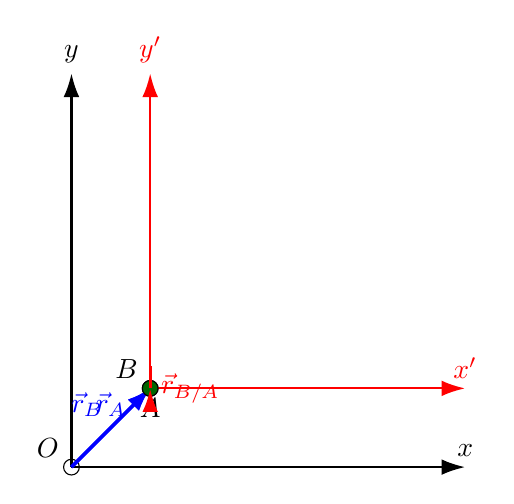
\begin{tikzpicture}[]

    \draw[] (0,0) circle [radius=1mm] node[left, above,xshift=-3mm] {$O$};
    
    \draw[-{Latex[length=3mm,width=2mm]}, thick, black] 
    (0,0) -- (5,0) node[left, above] {$x$};
    
    \draw[-{Latex[length=3mm,width=2mm]}, thick, black] (0,0) -- (0,5) node[left, above] {$y$};

    \draw[ fill=green!40!black] (\Ax,\Ay) circle [radius=1mm] node[right,below] {$A$};
        
    \draw[-{Latex[length=3mm,width=2mm]}, thick, red] 
    (\Ax,\Ay) -- ({\Ax+5,\Ay}) node[left, above] {$x^\prime$};
    
    \draw[-{Latex[length=3mm,width=2mm]}, thick, red] (\Ax,\Ay) -- ({\Ax,\Ay+5}) node[left, above] {$y^\prime$};

    \draw[-{Latex[length=3mm,width=2mm]}, very thick, blue] (0,0) -- (\Ax,\Ay) node[midway, above] {$\vec{r}_A$};

    \draw[-{Latex[length=3mm,width=2mm]}, very thick, blue] (0,0) -- (\Bx,\By) node[midway, above, xshift=-3mm] {$\vec{r}_B$};
    
    \draw[ fill=green!40!black] (\Bx,\By) circle [radius=1mm] node[left, above, xshift=-3mm] {$B$};

    \draw[-{Latex[length=3mm,width=2mm]}, very thick, red] (\Ax,\Ay) -- (\Bx,\By) node[midway, right] {$\vec{r}_{B/A}$};

\end{tikzpicture}


\end{document}
